%% LyX 2.3.3 created this file.  For more info, see http://www.lyx.org/.
%% Do not edit unless you really know what you are doing.
\documentclass[english]{article}
\usepackage[T1]{fontenc}
\usepackage[latin9]{inputenc}
\usepackage{babel}
\usepackage{amsmath}
\usepackage{amssymb}
\usepackage{setspace}
\usepackage[unicode=true,pdfusetitle,
 bookmarks=true,bookmarksnumbered=false,bookmarksopen=false,
 breaklinks=false,pdfborder={0 0 1},backref=section,colorlinks=false]
 {hyperref}
\hypersetup{
 hyperfootnotes=true}

\makeatletter

%%%%%%%%%%%%%%%%%%%%%%%%%%%%%% LyX specific LaTeX commands.
%% Because html converters don't know tabularnewline
\providecommand{\tabularnewline}{\\}

%%%%%%%%%%%%%%%%%%%%%%%%%%%%%% User specified LaTeX commands.
\usepackage{tikz}
\usepackage{braket}
\usepackage{qcircuit}
\usepackage{url}

\makeatother

\begin{document}
\title{Quantum Max Flow Analysis}
\author{Moreno Giussani}
\maketitle
\begin{abstract}
This document will describe the analysis I have performed in the last
months about the quantum implementation of the Max Flow algorithm.
The max flow problem involves finding a feasible flow through a single-source,
single-sink flow network that is maximum. I have been working for
finding a practical solution to this problem using a quantum algorithm
which could be at least as efficient as a classical one in a general
case. I achieved in implementing a quantum algorithm based on Grover's
algorithm which can solve the max flow problem, but its complexity
is much worse than a classical algorithm.
\end{abstract}
\tableofcontents{}

\pagebreak{}

\section{Introduction}

Before considering the algorithm, I have tried to understand most
of the concepts which lies behind a quantum algorithm.

For what regards quantum computing, the standard model of computation
is the quantum circuit. A quantum circuit is a scheme composed of
some elementary blocks, which are qubits and quantum logic gates.
Rows of this scheme represents qubits, while in columns are inserted
quantum logic gates.

Sometimes, the tensor network model is used, especially in quantum
physics papers.

\subsection{Qubit}

Qubits are the quantum equivalent of bits. They are usually represented
using the bra-ket notation. A single qubit $\Ket{Q_{0}}$is usually
described by a 2-dimensional column vector (Ket notation) which is
a specific linear combination of its orthonormal bases $\Ket{0}=\left[\begin{array}{c}
1\\
0
\end{array}\right]$ and $\Ket{1}=\left[\begin{array}{c}
0\\
1
\end{array}\right]$. When the qubit is measured (an equivalent operation of reading a
bit value in classical computing), its value collapses to either $\Ket{0}$
or $\Ket{1}$ (their orthonormal bases).

Suppose $\Ket{Q_{0}}$is defined as 
\[
\Ket{Q_{0}}=\alpha\Ket{0}+\beta\Ket{1}\;\alpha\in\mathbb{C},\beta\in\mathbb{C}
\]
Then $\alpha$ and $\beta$ must respect the rule $|\alpha|^{2}+|\beta|^{2}=1$
, because $|\alpha|^{2}$ represents the probability that a measurement
outputs $\Ket{0}$ and $|\beta|^{2}$ represents the probability that
a measurement outputs $\Ket{1}$. During the computation the qubit
can assume an ``overlapped'' state (both state 0 and state 1), but
when measured, its expressivity power reduces to a classical bit.
When both $\alpha$ and $\beta$ are different from 0 ,$Q_{0}$ is
said to be in superposition.

Qubits have also another interesting property: they cannot be copied.
There is no way to create an identical copy of an arbitrary unknown
quantum state (\textit{no cloning theorem}).

Now, things get a bit tricky when considering a N-qubit quantum computer.
If there are two or more qubits, their representation is made as the
Kronecker product of all of the qbits, so they often cannot be considered
as separated qubits. Suppose to have a 3-qubit quantum computer which
uses qubits $Q_{a},Q_{b},Q_{c}$. The representation of the state
of the quantum system becomes:

\begin{equation}
\Ket{Q_{x}}=x_{1}\left[\begin{array}{c}
1\\
0
\end{array}\right]+x_{2}\left[\begin{array}{c}
0\\
1
\end{array}\right]=\left[\begin{array}{c}
x_{1}\\
x_{2}
\end{array}\right]\;x\in\left\{ a,b,c\right\} 
\end{equation}

\begin{equation}
\Ket{Q_{ab}}=\Ket{Q_{a}}\otimes\Ket{Q_{b}}=\begin{bmatrix}a_{1}\begin{bmatrix}b_{1}\\
b_{2}
\end{bmatrix}\\
a_{2}\begin{bmatrix}b_{1}\\
b_{2}
\end{bmatrix}
\end{bmatrix}=\begin{bmatrix}a_{1}b_{1}\\
a_{1}b_{2}\\
a_{2}b_{1}\\
a_{2}b_{2}
\end{bmatrix}
\end{equation}

\begin{equation}
\Ket{Q_{ab}}=\begin{bmatrix}a_{1}b_{1}\\
a_{1}b_{2}\\
a_{2}b_{1}\\
a_{2}b_{2}
\end{bmatrix}=a_{1}b_{1}(\Ket{0}\otimes\Ket{0})+a_{1}b_{2}(\Ket{0}\otimes\Ket{1})+a_{2}b_{1}(\Ket{1}\otimes\Ket{0})+a_{2}b_{2}(\Ket{1}\otimes\Ket{1})
\end{equation}

\begin{equation}
\Ket{Q_{abc}}=\Ket{Q_{a}}\otimes\Ket{Q_{b}}\otimes\Ket{Q_{c}}=\Ket{Q_{ab}}\otimes\Ket{Q_{c}}=\begin{bmatrix}a_{1}b_{1}\begin{bmatrix}c_{1}\\
c_{2}
\end{bmatrix}\\
a_{1}b_{2}\begin{bmatrix}c_{1}\\
c_{2}
\end{bmatrix}\\
a_{2}b_{1}\begin{bmatrix}c_{1}\\
c_{2}
\end{bmatrix}\\
a_{2}b_{2}\begin{bmatrix}c_{1}\\
c_{2}
\end{bmatrix}
\end{bmatrix}=\begin{bmatrix}a_{1}b_{1}c_{1}\\
a_{1}b_{1}c_{2}\\
a_{1}b_{2}c_{1}\\
a_{1}b_{2}c_{2}\\
a_{2}b_{1}c_{1}\\
a_{2}b_{1}c_{2}\\
a_{2}b_{2}c_{1}\\
a_{2}b_{2}c_{2}
\end{bmatrix}
\end{equation}

In many cases it is impossible to consider $Q_{a},Q_{b}$and $Q_{c}$separately,
because in a quantum system some quantum logic gates may cause to
obtain a ``mixed'' state from which is not possible to find some
suitable $Q_{a},Q_{b}$and $Q_{c}$ which satisfies (4). This concept,
which is called \emph{entanglement}, will be described in detail later.
The quadratic sum of all elements of a Ket must be 1, like said before
for a single qubit.

\subsection{Quantum logic gates}

In a quantum circuit model, quantum logic gates are transformation
matrices which describes the behaviour of the physical quantum logic
gates. Quantum logic gates are represented by means of unitary square
matrices of size $2^{n}$,where $n$ is the number of qubits to which
a gate can be applied. A matrix $U$ is said unitary if

\[
UU^{\dagger}=U^{\dagger}U=I
\]

where $U^{\dagger}$ is the Hermitian transpose of $U$. The Hermitian
transpose can be obtained by transposing $U$ and then calculating
the complex conjugate of all elements in $U^{T}$ matrix.

The description of the state obtained from the application of a generic
quantum gate $G$from quantum state$\Ket{S^{0}}$ can be calculated
as:

\[
\Ket{S^{1}}=G\Ket{S^{0}}
\]

Some of the most known unitary logic gates are:
\begin{center}
\begin{tabular}{|c|c|c|c|}
\hline 
Name & Symbol & Matrix & Circuit\tabularnewline
\hline 
\hline 
Hadamard & $H$ & $\frac{1}{\sqrt{2}}\begin{bmatrix}1 & 1\\
1 & -1
\end{bmatrix}$ & \Qcircuit @C=1em @R=.7em {& \gate{H} & \qw}\tabularnewline
\hline 
Pauli-X (Not) & $X$(or $NOT$) & $\left[\begin{array}{cc}
0 & 1\\
1 & 0
\end{array}\right]$ & \Qcircuit @C=1em @R=.7em {& \gate{X} & \qw}\tabularnewline
\hline 
Pauli-Y & $Y$ & $\left[\begin{array}{cc}
0 & -i\\
i & 0
\end{array}\right]$ & \Qcircuit @C=1em @R=.7em {& \gate{Y} & \qw}\tabularnewline
\hline 
Pauli-Z & $Z$ or $R_{\pi}$ & $\left[\begin{array}{cc}
1 & 0\\
0 & -1
\end{array}\right]$ & \Qcircuit @C=1em @R=.7em {& \gate{Z} & \qw}\tabularnewline
\hline 
Swap & $SWAP$ & $\left[\begin{array}{cccc}
1 & 0 & 0 & 0\\
0 & 0 & 1 & 0\\
0 & 1 & 0 & 0\\
0 & 0 & 0 & 1
\end{array}\right]$ & \Qcircuit @C=1em @R=.7em {& \qswap & \qw  \\ & \qswap & \qw}\tabularnewline
\hline 
Controlled Not & $CNOT$ & $\left[\begin{array}{cccc}
1 & 0 & 0 & 0\\
0 & 1 & 0 & 0\\
0 & 0 & 0 & 1\\
0 & 0 & 1 & 0
\end{array}\right]$ & \Qcircuit @C=1em @R=.7em {& \ctrl{1} & \qw  \\ & \targ & \qw}\tabularnewline
\hline 
Toffoli & $CCNOT$ or $T$ & $\left[\begin{array}{cccccccc}
1 & 0 & 0 & 0 & 0 & 0 & 0 & 0\\
0 & 1 & 0 & 0 & 0 & 0 & 0 & 0\\
0 & 0 & 1 & 0 & 0 & 0 & 0 & 0\\
0 & 0 & 0 & 1 & 0 & 0 & 0 & 0\\
0 & 0 & 0 & 0 & 1 & 0 & 0 & 0\\
0 & 0 & 0 & 0 & 0 & 1 & 0 & 0\\
0 & 0 & 0 & 0 & 0 & 0 & 0 & 1\\
0 & 0 & 0 & 0 & 0 & 0 & 1 & 0
\end{array}\right]$ & \Qcircuit @C=1em @R=.7em {
  & \ctrl{2} \qw & \qw \\
  & \ctrl{1} \qw & \qw \\
  & \targ        & \qw  
}\tabularnewline
\hline 
Identity & $I$ & $\left[\begin{array}{cc}
1 & 0\\
0 & 1
\end{array}\right]$ & \Qcircuit @C=1em @R=.7em {& \qw &} or \Qcircuit @C=1em @R=.7em {& \gate{I} & \qw}\tabularnewline
\hline 
\end{tabular}
\par\end{center}

\begin{center}
When applied to a single qubit in one of its bases ($\Ket{0}$ or
$\Ket{1}$), an H gate will put the qubit in a superstate.
\par\end{center}

There are many more controlled gates which are represented using a
C prefix, like for the CNOT gate. Their structure is

\[
U=\left[\begin{array}{cccc}
u_{11} & u_{12} & ... & u_{1m}\\
u_{21} & u_{22} & ... & u_{2m}\\
... & ... & ... & ...\\
u_{m1} & u_{m2} & ... & u_{mm}
\end{array}\right]\:CU=\left[\begin{array}{ccccc}
1 & 0 & 0 & ... & 0\\
0 & 1 & 0 & ... & 0\\
0 & 0 & u_{11} & ... & u_{1m}\\
... & ... & ... & ... & ...\\
0 & 0 & u_{m1} & ... & u_{mm}
\end{array}\right]
\]

The ``measurement'' operator has symbol \Qcircuit @C=1em @R=.7em {& \meter &}

\subsection{Quantum circuits}

Quantum circuits can be represented via a ladder-like scheme. Each
row (horizontal lines) represents a distinct qubit, and the gates
which have to be applied to the given qubit are inserted on that line,
from left to right. Gates on the same column has to be applied at
the same time.

Here's an example with a 2-qubit circuit:

\begin{align*}\Qcircuit @C=1em @R=.7em {
\Ket{Q_0} & & \gate{H} & \gate{Z} & \gate{H} & \ctrl{1} & \gate{H}  & \qw & \meter \\
\Ket{Q_1} & & \qw      & \gate{X} & \qw      & \targ    & \gate{H} & \qw & \meter
}\end{align*}

which is equivalent to the given circuit:

\begin{align*}\Qcircuit @C=1em @R=.7em {
\Ket{Q_0} & & \gate{H} & \gate{Z} & \gate{H} & \ctrl{1} & \gate{H}  & \gate{I} & \meter \\
\Ket{Q_1} & & \gate{I} & \gate{X} & \gate{I} & \targ    & \gate{H}  & \gate{I} & \meter
}\end{align*}

Identity gates columns will not change the state, they can be ignored,
because

\[
I_{n\,x\,n}\otimes I_{m\,x\,m}=I_{nm\,x\,nm}
\]

As said before, in a multi qubit computer, considering $Q_{0}$and
$Q_{1}$as independent qubits would often lead to mistakes, because
the application of a gate to a qubit would cause some side effects
on other qubits.

If not specified, like in this case, every qubit is conventionally
initialized to state $\Ket{0}$. 

Knowing that the above circuit is a 2-qubit circuit, the initial state
$\Ket{S^{0}}$is described as $\Ket{Q_{0}}\otimes\Ket{Q_{1}}=\Ket{00}$
.

Then, the applied gate is 

\[
H\otimes I=\left[\begin{array}{cccc}
\frac{1}{\sqrt{2}} & 0 & \frac{1}{\sqrt{2}} & 0\\
0 & \frac{1}{\sqrt{2}} & 0 & \frac{1}{\sqrt{2}}\\
\frac{1}{\sqrt{2}} & 0 & -\frac{1}{\sqrt{2}} & 0\\
0 & \frac{1}{\sqrt{2}} & 0 & -\frac{1}{\sqrt{2}}
\end{array}\right]
\]
.

So, the state of the circuit after the application of $H\otimes I$
is:

\[
\Ket{S^{1}}=(H\otimes I)\Ket{S^{0}}=\left[\begin{array}{cccc}
\frac{1}{\sqrt{2}} & 0 & \frac{1}{\sqrt{2}} & 0\\
0 & \frac{1}{\sqrt{2}} & 0 & \frac{1}{\sqrt{2}}\\
\frac{1}{\sqrt{2}} & 0 & -\frac{1}{\sqrt{2}} & 0\\
0 & \frac{1}{\sqrt{2}} & 0 & -\frac{1}{\sqrt{2}}
\end{array}\right]\left[\begin{array}{c}
1\\
0\\
0\\
0
\end{array}\right]=\left[\begin{array}{c}
\frac{1}{\sqrt{2}}\\
0\\
\frac{1}{\sqrt{2}}\\
0
\end{array}\right]=\frac{1}{\sqrt{2}}\Ket{00}+\frac{1}{\sqrt{2}}\Ket{10}
\]

Now, simulating the whole execution:

\[
\Ket{S^{2}}=(Z\otimes X)\Ket{S^{1}}=\left[\begin{array}{cccc}
0 & 1 & 0 & 0\\
1 & 0 & 0 & 0\\
0 & 0 & 0 & -1\\
0 & 0 & -1 & 0
\end{array}\right]\left[\begin{array}{c}
\frac{1}{\sqrt{2}}\\
0\\
\frac{1}{\sqrt{2}}\\
0
\end{array}\right]=\left[\begin{array}{c}
\frac{1}{\sqrt{2}}\\
0\\
0\\
-\frac{1}{\sqrt{2}}
\end{array}\right]
\]

\[
\Ket{S^{3}}=(H\otimes I)\Ket{S^{2}}=\left[\begin{array}{cccc}
\frac{1}{\sqrt{2}} & 0 & \frac{1}{\sqrt{2}} & 0\\
0 & \frac{1}{\sqrt{2}} & 0 & \frac{1}{\sqrt{2}}\\
\frac{1}{\sqrt{2}} & 0 & -\frac{1}{\sqrt{2}} & 0\\
0 & \frac{1}{\sqrt{2}} & 0 & -\frac{1}{\sqrt{2}}
\end{array}\right]\left[\begin{array}{c}
\frac{1}{\sqrt{2}}\\
0\\
0\\
-\frac{1}{\sqrt{2}}
\end{array}\right]=\left[\begin{array}{c}
\frac{1}{2}\\
-\frac{1}{2}\\
\frac{1}{2}\\
\frac{1}{2}
\end{array}\right]
\]

\[
\Ket{S^{4}}=CNOT\Ket{S^{3}}=\left[\begin{array}{cccc}
1 & 0 & 0 & 0\\
0 & 1 & 0 & 0\\
0 & 0 & 0 & 1\\
0 & 0 & 1 & 0
\end{array}\right]\left[\begin{array}{c}
\frac{1}{2}\\
-\frac{1}{2}\\
\frac{1}{2}\\
\frac{1}{2}
\end{array}\right]=\left[\begin{array}{c}
\frac{1}{2}\\
-\frac{1}{2}\\
\frac{1}{2}\\
\frac{1}{2}
\end{array}\right]
\]

\[
\Ket{S^{5}}=(H\otimes H)\Ket{S^{4}}=\left[\begin{array}{cccc}
\frac{1}{2} & \frac{1}{2} & \frac{1}{2} & \frac{1}{2}\\
\frac{1}{2} & -\frac{1}{2} & \frac{1}{2} & -\frac{1}{2}\\
\frac{1}{2} & \frac{1}{2} & -\frac{1}{2} & -\frac{1}{2}\\
\frac{1}{2} & -\frac{1}{2} & -\frac{1}{2} & \frac{1}{2}
\end{array}\right]\left[\begin{array}{c}
\frac{1}{2}\\
-\frac{1}{2}\\
\frac{1}{2}\\
-\frac{1}{2}
\end{array}\right]=\left[\begin{array}{c}
0\\
1\\
0\\
0
\end{array}\right]
\]

\[
\Ket{S^{6}}=(I\otimes I)\Ket{S^{5}}=\Ket{S^{5}}=\left[\begin{array}{cccc}
1 & 0 & 0 & 0\\
0 & 1 & 0 & 0\\
0 & 0 & 1 & 0\\
0 & 0 & 0 & 1
\end{array}\right]\left[\begin{array}{c}
0\\
1\\
0\\
0
\end{array}\right]=\left[\begin{array}{c}
0\\
1\\
0\\
0
\end{array}\right]
\]

Then, the measurement would show $\Ket{01}$as final result ($Q_{0}=0,Q_{1}=1$).

By definition, all the quantum gates that have been applied to this
circuit are unitary. For this, by replacing recursively $S^{i},\:0<i<6$
with $S^{i-1}$ in the example circuit we obtain:

\[
\Ket{S^{6}}=(I\otimes I)(H\otimes H)CNOT(H\otimes I)(Z\otimes X)(H\otimes I)\Ket{S^{0}}
\]

So, if the circuit is unitary, then we could reverse the execution
from the final state to the initial one. This property is called reversibility.
In the example:

\[
[(I\otimes I)(H\otimes H)CNOT(H\otimes I)(Z\otimes X)(H\otimes I)]^{-1}\Ket{S^{6}}=\Ket{S^{0}}
\]

\[
[(I\otimes I)(H\otimes H)CNOT(H\otimes I)(Z\otimes X)(H\otimes I)]^{\dagger}\Ket{S^{6}}=\Ket{S^{0}}
\]

\[
\Ket{S^{0}}=(H\otimes I){}^{\dagger}(Z\otimes X){}^{\dagger}(H\otimes I){}^{\dagger}CNOT{}^{\dagger}(H\otimes H){}^{\dagger}(I\otimes I){}^{\dagger}\Ket{S^{6}}
\]

In our example, there are no complex gates, so

\[
\Ket{S^{0}}=(H\otimes I)'(Z\otimes X)'(H\otimes I)'CNOT'(H\otimes H)'(I\otimes I)'\Ket{S^{6}}
\]

All the applied matrices are symmetrical, so

\[
\Ket{S^{0}}=(H\otimes I)(Z\otimes X)(H\otimes I)CNOT(H\otimes H)(I\otimes I)\Ket{S^{6}}
\]

This means that from every state of the system, we could rewind the
execution flow. This property is called \emph{reversible computing}
and it is a property of every quantum computing algorithm. In this
case, we can also build a circuit that from the final state $S^{6}$could
reobtain the initial state $S^{0}.$ The circuit that allows to do
that is the original circuit flipped horizontally, that is:

\begin{align*}\Qcircuit @C=1em @R=.7em {
\Ket{0} & &  \gate{I} & \gate{H} & \ctrl{1} & \gate{H} & \gate{Z} & \gate{H} & \meter \\
\Ket{1} & &  \gate{I} & \gate{H} & \targ    & \gate{I} & \gate{X} & \gate{I} & \qw &\meter
}\end{align*}

\begin{spacing}{3}
Sometimes, considering qubits as independent from others would cause
mistakes. Consider the following simple circuit:
\end{spacing}

\begin{align*}\Qcircuit @C=1em @R=.7em {
\Ket{Q_0} & &  \gate{H} & \gate{I} & \ctrl{1} & \meter \\
\Ket{Q_1} & &  \gate{H} & \gate{H} & \targ    & & \meter
}\end{align*}

\[
\Ket{S^{0}}=\Ket{00}
\]

\[
\Ket{S^{1}}=H\otimes H\Ket{S^{0}}=\left[\begin{array}{cccc}
\frac{1}{2} & \frac{1}{2} & \frac{1}{2} & \frac{1}{2}\\
\frac{1}{2} & -\frac{1}{2} & \frac{1}{2} & -\frac{1}{2}\\
\frac{1}{2} & \frac{1}{2} & -\frac{1}{2} & -\frac{1}{2}\\
\frac{1}{2} & -\frac{1}{2} & -\frac{1}{2} & \frac{1}{2}
\end{array}\right]\left[\begin{array}{c}
1\\
0\\
0\\
0
\end{array}\right]=\left[\begin{array}{c}
\frac{1}{2}\\
\frac{1}{2}\\
\frac{1}{2}\\
\frac{1}{2}
\end{array}\right]
\]

\[
\Ket{S^{2}}=I\otimes H\Ket{S^{1}}=\left[\begin{array}{cccc}
\frac{1}{\sqrt{2}} & \frac{1}{\sqrt{2}} & 0 & 0\\
\frac{1}{\sqrt{2}} & -\frac{1}{\sqrt{2}} & 0 & 0\\
0 & 0 & \frac{1}{\sqrt{2}} & \frac{1}{\sqrt{2}}\\
0 & 0 & \frac{1}{\sqrt{2}} & -\frac{1}{\sqrt{2}}
\end{array}\right]\left[\begin{array}{c}
\frac{1}{2}\\
\frac{1}{2}\\
\frac{1}{2}\\
\frac{1}{2}
\end{array}\right]=\left[\begin{array}{c}
\frac{1}{\sqrt{2}}\\
0\\
\frac{1}{\sqrt{2}}\\
0
\end{array}\right]=\frac{1}{\sqrt{2}}\Ket{00}+\frac{1}{\sqrt{2}}\Ket{10}
\]

\[
\Ket{S^{3}}=CNOT\Ket{S^{2}}=\left[\begin{array}{cccc}
1 & 0 & 0 & 0\\
0 & 1 & 0 & 0\\
0 & 0 & 0 & 1\\
0 & 0 & 1 & 0
\end{array}\right]\left[\begin{array}{c}
\frac{1}{\sqrt{2}}\\
0\\
\frac{1}{\sqrt{2}}\\
0
\end{array}\right]=\left[\begin{array}{c}
\frac{1}{\sqrt{2}}\\
0\\
0\\
\frac{1}{\sqrt{2}}
\end{array}\right]=\frac{1}{\sqrt{2}}\Ket{00}+\frac{1}{\sqrt{2}}\Ket{11}
\]

In state $S^{3}$, the two qubits are no more independent from eachother.
In state $S^{1}$, both $\Ket{Q_{0}}$ and $\Ket{Q_{1}}$ are in state
$\frac{1}{\sqrt{2}}(\Ket{0}+\Ket{1})$, then in $S^{2}$, $\Ket{Q_{1}}=\Ket{0}$and
$\Ket{Q_{0}}=\frac{1}{\sqrt{2}}(\Ket{0}+\Ket{1})$. In $S^{3}$ it
is nonsensical considering the two qubits individually. They can be
both 0 or both 1 with equal probability. When two or more qubits are
dependent on eachother, it is said that they are \emph{entangled}.
If we measure $Q_{0}$ as first, its measurement will influence $Q_{1}$'s
measurement, because if and only if $Q_{0}$ collapses to $\Ket{0}$,
then $Q_{1}$ will collapse to $\Ket{0}$. 

In the\emph{ CHSH game} is proven that when one of two entangled quantum
particles (which are modeled as qubits in circuits) is measured, the
other particle will assume the same state that the first particle
had assumed when collapsing, at a faster-than-light speed.

\subsection{Tensor Network Diagrams}

Tensor network diagrams are models used to better represent complex
entangled circuits, because they allow to define circuits with less
parameters. They are usually lossy data compression methods used for
describing the most important properties of the quantum state of a
system. Quantum circuits are submodels of tensor network diagrams.

A tensor is usually a box, oval or triangle with some wires pointing
up and down. Wires pointing up are called arms, while wires pointing
down are called legs. Arms are upper indices while legs are lower
indices. The number of arms and legs determines the underlying algebraic
structure (scalar, vector or matrix in our context). They are often
tilted by 90 degrees clockwise. Vectors are single arm tensors, while
matrices has one arm and one leg.

Disconnected tensors are multiplied using the tensor product (Kronecker
product in our case). Tensors can be freely moved past eachother (plannar
deformation) without changing the semantic of the content they model,
as in the example:

\begin{align*}\Qcircuit @C=1em @R=.7em {
&  \gate{A} & \qw & \\
&  \qw & \gate{B} &}
=
\Qcircuit @C=1em @R=.7em {
&  \gate{A} & \qw & \\
&  \gate{B} & \qw &}
=
\Qcircuit @C=1em @R=.7em {
&  \gate{B} & \qw & \\
&  \qw & \gate{A} &}
\end{align*}

Unlike quantum circuits, wires can cross tensor symbols and other
wires as long as the wire endpoints do not change.

Two tensors connected together means that they are multiplied (contracted
or summed over). The following image

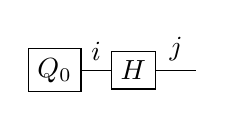
\begin{tikzpicture}     
\node[draw, shape=rectangle] (v0) at (0,0) {$Q_0$};
\node[draw, shape=rectangle] (v1) at (1,0) {$H$};
\node [coordinate] (end) [right of=v1, node distance=0.8cm]{};
\draw (v0) -- node[above]{$i$} (v1) ;
\draw  (v1) -- node[above]{$j$} (end) ;     \end{tikzpicture} 
= 
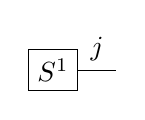
\begin{tikzpicture}     
\node[draw, shape=rectangle] (v0) at (0,0) {$S^1$};
\node [coordinate] (end) [right of=v0, node distance=0.8cm]{};
\draw  (v0) -- node[above]{$j$} (end) ;     \end{tikzpicture} 

Is equivalent to

\[
S^{1}=Q_{0}H
\]

Tensor network diagrams were used in \cite{1}.

A more complete and better explanation can be found in \cite{2-1}.

\section{The classical algorithm}

Classical maximum flow algorithms are based of the Ford-Fulkerson
method via Edmonds-Karp algorithm and Dinic's algorithm.

A maximum flow algorithm is an algorithm which attempts to find a
feasible flow which is maximum.

\subsection{Ford-Fulkerson method / Edmonds-Karp algorithm}

Ford-Fulkerson method\cite{3} requires as input:
\begin{itemize}
\item A network graph $G(V,E)$ where $V$ is the vertices set and $E$
is the edges set 
\item $\forall(u,v)\in E:\exists f(u,v)$ where $f(u,v)$ is the flow on
the edge from vertex $u$ to vertex $v$
\item $\forall(u,v)\in E:\exists c(u,v)$ where $c(u,v)$ is the available
capacity of the edge from vertex $u$ to vertex $v$
\item A source node $s\in V$ and a sink node $t\in V$
\item Some constraints:
\begin{itemize}
\item Capacity constraints: $\forall(u,v)\in E:f(u,v)\leq c(u,v)$
\item Skew symmetry: $\forall(u,v)\in E:f(u,v)=-f(v,u)$
\item Flow conservation: $\forall u\in V:\:u\ne s\:and\:u\ne t\implies\sum_{w\in V}f(u,w)=0$
\item Source and sink flow constraint: $\sum_{(s,u)\in E}f(s,u)=\sum_{(v,t)\in E}f(v,t)$
\end{itemize}
\item A residual network graph $G_{f}(V,E_{f})$ with (residual) capacity
$c_{f}(u,v)=c(u,v)-f(u,v)$ and no flow. A residual graph has some
important properties. If $f(u,v)>0$ and $c(v,u)=0$, then $c_{f}(v,u)=c(v,u)-f(u,v)=f(u,v)>0$
, so a possible flow can be present in a residual graph but not in
the original graph $G$ 
\end{itemize}
Ford-Fulkerson method is composed of the following steps:
\begin{enumerate}
\item $\forall(u,v)\in E:\:f(u,v)=0$
\item While there is a path $P\subseteq E:P\ne\emptyset$ from $s$ to $t$
in $G_{f}$with $c_{f}(u,v)>0\;\forall(u,v)\in P$
\begin{enumerate}
\item Find $c_{f}(P)=min\{c_{f}(u,v):(u,v)\in P\}$
\item $\forall(u,v)\in P:$
\begin{enumerate}
\item $f(u,v)=f(u,v)+c_{f}(P)$ (send the flow along the path)
\item $f(v,u)=f(v,u)-c_{f}(P)$ (reduce the flow in the ``reversed'' path)
\end{enumerate}
\end{enumerate}
\end{enumerate}
Step 2 looks for an augmenting path (by using a search algorithm),
then step 2.a finds the maximum admissible flow correction that can
be done in path P , then step 2.b updates the flows.

Edmond-Karps algorithm applies the Ford-Fulkerson method by implementing
a breadth-first search to find the path in step 2. By using breadth
first, the complexity of the algorithm is $\mathcal{O}(VE^{2})$

\subsection{Dinitz's algorithm}

Dinitz's algorithm (better known as Dinic's algorithm) is very similar
to Edmond-Karps, it uses too a residual graph and looks for an augmenting
path by using a level graph. A \emph{level graph} is a graph that
assigns to each vertex its distance to the root node. In some paper,
it is called \emph{layer graph}.

Dinitz's algorithm steps are:
\begin{enumerate}
\item Building the residual graph
\item Building the layer graph from the residual graph, by discarding edges
connecting vertices at the same level.
\item All the paths in the layer graph contain augmenting paths. If there
are no paths, the flow is maximum.
\item Update the flows and the residual graph
\item Go to step 2
\end{enumerate}

\section{Quantum Implementation}

Before analyzing the proposed quantum implementations, there are some
important details that has to be described about the actual state
of the art of quantum computers.

For what regards the chosen quantum algorithm, I have considered many
options. The most important specification that I have considered is
that the quantum max flow algorithm implementation must work on a
generic directed weighted graph, because classical computers can still
provide excellent results for more specific cases.

\subsection{Quantum Computers}

Quantum computers at the actual state of the technology cannot provide
a memory or either a ``qRAM'', because there is no way to reproduce
an arbitrary unknown state (no cloning theorem) and there is no known
way to store and load qubits (at least, \href{https://www.nextbigfuture.com/2018/12/ionq-has-the-most-powerful-quantum-computers-with-79-trapped-ion-qubits-and-160-stored-qubits.html}{not confirmed from reliable sources}).
All the qubits has to be allocated at the beginning of the computation
and there is no ``discard'' option for a qubit.

At the moment, the most powerful quantum computer has more or less
70 qubits available (\href{https://ai.googleblog.com/2018/03/a-preview-of-bristlecone-googles-new.html}{Google Bristlecone})

The whole circuit has to be available at compile time, and there is
a unique flow of execution. Measurement cannot be used to change the
behaviour of the quantum system at runtime. 

Quantum states are very unstable, so this makes the process of creating
a qRAM even more complex.

From a programmer's point of view, a quantum computer programming
is very similar to FPGA programming.

Quantum computers have a structure very similar to vector machines
and GPUs, but without any buffer or memory. For this reason, they
have been successfully applied in \href{https://ai.googleblog.com/2018/12/exploring-quantum-neural-networks.html}{neural networks},
an application where GPUs excels at.

Quantum computers provides a probabilistic result, circuits are run
many times and can be used for critical systems only if their results
can be checked by classical computers or other more reliable methods.

Quantum gates has a reliability percentage, for this reason long circuits
tend to fail in producing correct results.

In most quantum computers, not all qubits lines are interconnected.
Most qubits are interconnected with 2 or more other qubits.

\subsection{Tensor Networks}

In \cite{1}, it is proposed to represent flow graphs as tensor networks,
where the capacity of each link in the flow network is represented
as the dimension of a Hilbert space. This implementation looked very
complex, and also relies on qudits (quantum digits), so the required
size of the circuit for representing a simple graph could explode. 

A qudit is a quantum information unit with n orthonormal bases, and
the superposition is between all n states. For n=2, a qudit is exactly
equivalent to a qubit. Qudits may have more expressive power than
qubits due to the availability of more superposition states.

Also, the paper does not provide an implementation of the actual circuit,
which led me to look for other options.

\subsection{Other attempts}

I have thought about algorithms which could exploit at most as possible
the quantum potential, instead of ``porting'' classical algorithms
to quantum. The first critical problems which arised were:
\begin{enumerate}
\item How to represent graphs? 
\item How to represent weights?
\end{enumerate}

\paragraph*{How to represent graphs}

I tried to find a smart way to represent graphs in quantum circuits.
I took inspiration from \cite{1} in which they attempt to represent
a graph as a tensor network. Knowing that quantum circuits are submodels
of tensor networks, I attempted to represent a simple tree architecture
(without weights) in the circuit. I used qubits as nodes and entanglement
to represent edges between nodes. I accomplished in representing a
single simple path without repeating nodes (which is indeed a trivial
problem), which would have been either taken or not taken, but I failed
in representing more complex structures, due to the fact that i haven't
been able to entangle 3 qubits together. This attempt seemed promising
to me because with entanglement i would have obtained the flow constraint,
so that if a node is ``taken'', then another following node should
be taken too. If we consider for example the state $\frac{1}{\sqrt{2}}(\Ket{00}+\Ket{11})$,
if the first qubit is taken, then the following one would be taken
too or none of those would be taken.

\paragraph{How to represent weights}

In the upper representation there is no weight representation. Weights
are hard to be represented in a quantum environment, especially because
comparisons in quantum circuits (eg toffoli) are hard to implement
and cause an explosion in size of the circuit. What I have considered
is to represent only the layer graph built on the residual graph in
the quantum circuit. Then, I would have used the quantum circuit to
find a path in the classical residual graph to obtain a (small) speedup. 

\subsection{Quantum Edmond-Karps Algorithm}

In \cite{key-10} is shown an approach for building a quantum max
flow algorithm, which is better explained in \cite{key-9}. They propose
to build a layered subgraph (also called level subgraph, the same
that is used in Dinitz's algorithm). This is the version that iI have
implemented. The procedure is:
\begin{enumerate}
\item Set the level $l$ to $\infty$ to all nodes except the source $s$,
whose level is set to 0.
\item Create a one entry queue $Q=$\{$s$\}
\item While $Q\neq\emptyset$
\begin{enumerate}
\item Take the first node $n$ from $Q$
\item Find by Grover\textquoteright s search all its neighbors $y$ with
$l(y)=\infty$, set $l(y)=l(n)+1$, and append $y$ into $Q$
\item Remove $n$ from $Q$
\end{enumerate}
\end{enumerate}
But there is a problem with this algorithm, at step 3.b. It can become
clear after Grover's algorithm is being explained.

\subsubsection{Grover's algorithm}

Before defining what does Grover's algorithm , it is necessary defining
what is a quantum oracle.

A \emph{quantum oracle} of a function $f(C)$ is a quantum circuit
which given an input $S$, it outputs $\Ket{1}$ on a specific qubit
if $S\in f(C)$, $\Ket{0}$otherwise. Grover's algorithm has complexity
$O({\sqrt{N}})$ times the oracle complexity.

Grover's algorithm \cite{key-11}(sometimes called Grover's search
algorithm) is a quantum algorithm which, given as input a oracle of
$f(C)$ and the expected output of the function $S$, it attempts
to find an input $C\in f^{-1}(S)$ which could have generated $S$.
This has some important consequences in cryptography, because many
algorithms for cryptography could possibly be broken if a quantum
representation of the cryptographic one way function is provided. 

Originally, Grover's algorithm was called Grover's search, because
it allows to do a search in an unsorted database of possible inputs.
But knowing that building (classically) such a oracle for a unsorted
database requires at least linear complexity, it is not suggested
to be used practically for searches. This is the main reason which
blocks the provided quantum algorithm to outcome the classical one.

Grover's algorithm outputs one result per run. It could be scaled
both horizontally (another quantum computer running the same circuit)
and vertically (double the quantum circuit, like in a distinct quantum
computer). 

Grover's circuit is composed of four parts, superposition initialization,
oracle, phase shift and diffusion.

\begin{align*}\Qcircuit @C=1em @R=0em { 
&\multigate{2}{\mathcal{H}}&\qw&\multigate{2}{Oracle}& \qw & \qw & \multigate{2}{\mathcal{H}}&\qw &\multigate{2}{Phase\:shift}& \qw & \multigate{2}{\mathcal{H}}&\qw    \\
&\ghost{\mathcal{H}}&       \qw&\ghost{Oracle}& \qw & \qw & \ghost{\mathcal{H}}& \qw& \ghost{Phase\:shift}& \qw & \ghost{\mathcal{H}}& \qw     \\ 
&\ghost{\mathcal{H}}&       \qw&\ghost{Oracle}& \qw & \qw & \ghost{\mathcal{H}}& \qw& \ghost{Phase\:shift}& \qw& \ghost{\mathcal{H}}& \qw     \\
& \dstick{superposition}\cwx[-1] &&&&&&& \dstick{diffusion}\cwx[-1] \gategroup{1}{7}{3}{11}{.7em}{--}
} \end{align*}

\:

Of those parts, the oracle and the diffusion part are iterated many
times. The number of times that they have to be repeated has to be
set as $\frac{\pi}{4}\sqrt{2^{n}}$, where $n$ is the number of qubits
used ( $2^{n}$is the size of the ``database''). The problem is
that $\frac{\pi}{4}\sqrt{2^{n}}$ is often not an integer. Rounding
the number of iterations could cause to not find a solution even when
it exists.
\begin{quote}
\begin{center}
\textquotedblleft Grover\textquoteright s quantum searching technique
is like cooking a souffl�. You put the state obtained by quantum parallelism
in a \textquotedblleft quantum oven\textquotedblright{} and let the
desired answer rise slowly. Success is almost guaranteed if you open
the oven at just the right time. But the souffl� is very likely to
fall---the amplitude of the correct answer drops to zero---if you
open the oven too early.\textquotedblright{} -- Kristen Fuchs \cite{key-11}
\par\end{center}
\end{quote}

\subsubsection{Finding neighbors by Grover's algorithm}
\begin{quote}
3.b) Find by Grover\textquoteright s search all its neighbors $y$
with $l(y)=\infty$, set $l(y)=l(n)+1$, and append $y$ into $Q$
\end{quote}
This is the key point. Grover's algorithm for searches returns one
result per run, which is chosen casually between all the possible
results. Finding all the infinite-distanced neighbors of a single
node is a task that can be done in $O(\frac{\pi}{4}\sqrt{2^{\left\lceil \log_{2}\bar{b}\right\rceil }}\bar{b})\implies O(\bar{b}\sqrt{\bar{b}})$,
where $\bar{b}$ is the average number of neighbors in the graph (``branching
factor'').

The explanation behind $O(\frac{\pi}{4}\sqrt{2^{\left\lceil \log_{2}\bar{b}\right\rceil }}\bar{b})$
lies in the fact that the algorithm has to be rerun at least $\bar{b}$
(neighboring nodes) time to find all infinite distance neighbors,
and each run has to do $\frac{\pi}{4}\sqrt{2^{\left\lceil \log_{2}\bar{b}\right\rceil }}$
iterations, where $2^{\left\lceil \log_{2}\bar{b}\right\rceil }$
is the size of the database (``search space''). The number of database
entries has to be a power of 2. The assumption behind this estimation
is that the best ``lucky'' case is considered, no unexpected outcomes
are considered.

The overall quantum complexity is then 

\[
O(\bar{b}^{\frac{3}{2}}N)
\]

where $N$is the number of nodes in the graph. This complexity can
be reduced heavily depending on the topology of the network. Considering
the average branching factor as $\bar{b}=\frac{E}{N}$ where $E$
is the number of edges in the network flow graph, we get:

\[
O(\frac{E^{\frac{3}{2}}}{\sqrt{N}})
\]

This complexity has to be multiplied with the complexity of the oracle.
A boolean oracle (the only one which could work in a general network
flow graph) has almost constant complexity. The problem is that the
oracle has to be built classically. This can be done in $O(\bar{b})=O(\frac{E}{N})$.
Unfortunately, when a node is found, a layer is assigned to it, the
database changes and so the oracle has to be changed (recomputed classically)
too. Each element can be found at most once (once it is found, it
gets its layer number updated), so the overall complexity (both classical
and quantum) is:

\[
O(\frac{E^{\frac{3}{2}}}{\sqrt{N}}\cdot\frac{E}{N}\cdot N)=O(\frac{E^{\frac{5}{2}}}{\sqrt{N}})
\]

This result is still optimistic, because there is a strong assumption
behind this estimation. Quantum unexpected outcomes happens very often,
especially in large sparse search spaces. This is due to the intrinsic
nature of quantum computers and it is due to the problem of having
many values to be searched. Quantum unexpected outcomes happen because
the probability of some values which shouldn't be found is not exactly
zero, and tend to increase as the size of the search space increases. 

Suppose that we have a dataset of 200 elements where 50 elements are
being searched. Then, we would have an 8 qubit quantum circuit in
which 56 entries are out of bound, 100 elements have 1\% each chance
to be extracted and 100 elements shouldn't be found. Noise in a quantum
algorithm can substantially increase the chances to outcome erroneous
values, also because each iteration in Grover's algorithm amplifies
the most significant possible outcomes, which could be an erroneous
one (noise).

\[
\]

The complexity considered in \cite{key-9} is based on an ``adjacency
model''. The adjacency model I suppose is based on an adjacency matrix,
which could used to store information about the network. 

Implementing such a matrix in a quantum circuit would cause to have
huge circuits. Let's start by a graph without network capacities.
Then we would have a circuit with a size of $N^{2}$ qubits. Actually,
this would be unfeasible for most networks due to the fact that the
most powerful quantum computer can work on at most 100 qubits.

\subsubsection{Building the oracle}

Building the oracle requires to know where the elements are in the
classical dataset. This means that to know where they are, a linear
search (if the set is unordered) has to be performed. Once the elements
have been found, it is nonsensical insert them into an oracle and
then let the quantum algorithm find the values that have been inserted
in the oracle, because we still know what we have to search. It could
have sense only for testing how a quantum computer behaves, so this
is the reason why I have kept writing the implementation. 

\subsection{Actual implementation}

The actual implementation sticks as most as possible to the quantum
Edmond-Karps Algorithm version. The algorithm must have a classical
part and a quantum part which must work together. The classical part
is written in C\#, while the quantum part is written in Q\# and they
work together by using Microsoft Quantum Development Kit. 

The quantum implementation uses Grover's algorithm to find neighbors
whose distance is infinite. The Grover's algorithm implementation
is the one provided with the quantum templates of Microsoft QDK. Neighbors
are represented as indices, which has to be found in the implicit
database. An\emph{ implicit database }is a database in which all the
possible elements are present. The elements which has to be found
are marked. Non-marked elements should never be outcomed.

To improve slightly the algorithm's performance, the algorithm stops
layering the graph once the sink is found. It also excludes the nodes
whose flow cannot be increased from the layering phase.

Then, from the sink, the path is rewinded to the source (it is a spanning
tree) and then the flow is augmented on the path. The algorithm stops
when the layered graph cannot include the sink.

It also includes a random graph generator for generating samples.
To provide a graphical output of the result, the graph is being outputted
as .dot and .gexf. The README.md file contains the technical details
for building and testing the program. 

On Linux, a .png file is also generated from the .dot.

The program outputs and saves to file also the number of unexpected
outcomes found during the execution.

\paragraph*{Project structure}

The project is composed of 3 C\# files, a .csproj configuration XML
file and a Q\# file, that is the Microsoft Quantum's \href{https://github.com/microsoft/Quantum/blob/master/Samples/src/DatabaseSearch/DatabaseSearch.qs}{Grover Algorithm implementation}.

The ``main'' C\# file is Driver.cs, which contains two classes,
Utilities and Driver.

Utilities contains code for generating a graph schema, while Driver
contains the main function and the code that calls the quantum Edmonds-Karp
algorithm.

Graph.cs contains the code for generating and handling graphs. It
has 3 classes, Edge, Graph and Node.

Graph.addLayer is the layering function, while Graph.findInnerPath
is the recursive function that looks for an augmenting path. The quantum
function is Graph.findLayerNeighbors, which is used both to find infinite
distanced neighbors (infinite value is stored as -1) and to find the
augmenting path.

\section{Programming environment}

The chosen programming enviroment for the algorithm implementation
is Microsoft Quantum Development Kit (QDK) on Visual Studio Code.

Visual Studio Code is one of the \href{https://insights.stackoverflow.com/survey/2018\#development-environments-and-tools}{most popular development environments},
due to its simple design. It is composed of a simple but powerful
lightweight editor, with many extensions available for download. This
allows the developer to install packages as soon as they are required,
which is a great advantage. It offers an intuitive UI similar to Atom
IDE but much lighter and reactive. 

QDK requires C\# code for the classical parts and Q\# (which is similar
to F\# and C\#) code for the quantum parts. The QDK has many useful
libraries, a compiler and a simulator which could be run very easily
from Visual Studio Code.

The QDK is still under development, it is updated with a new version
almost monthly but updates often break older versions' code. It is
based on Microsoft .Net and it is cross-platform.

QDK is documented, but the documentation is sparse in many Microsoft
websites, and not all articles are updated. Anyway, the Microsoft
Quantum team is always available on Github and updates the outdated
documentation as soon as they have been notified of.

There are also many Microsoft based examples/libraries, such as an
Grover's algorithm implementation which i used in the implemented
project.

There are also some Q\# community integrations which allow to integrate
the Q\# code to other quantum languages, such as Qiskit and OpenQasm.

\part*{Conclusion}

The quantum algorithm implementation does not show an advantage with
respect to a classical algorithm such as Dinitz's or Edmonds-Karp.
The quantum implementation can be useful to see how often unexpected
outcomes do happen in a much simplified quantum algorithm (the quantum
oracle implementation is the simplest possible). The implemented algorithm
is the implementation of the analysed algorithm described on \cite{key-10}.
It is very inefficient, due to the complexity required to encode a
quantum oracle and the scarcity of qubits in quantum computers (storing
a complete graph in a quantum oracle requires too many qubits). To
obtain a quantum speedup, it is required to not convert classical
algorithms into quantum ones, because classical computation has different
properties with respect to quantum computation, because operations
which are simple in classical computing (such as comparing two bits)
can be very complex in quantum and viceversa. Exploiting quantum circuits'
capabilities is a very challenging task, due to the logic behind the
quantum gates and the qubits' properties.

\pagebreak{}
\begin{thebibliography}{1}
\bibitem{1}Shawn X. Cui, Michael H. Freedman, Or Sattath, Richard
Stong: \textquotedblleft Quantum Max-flow/Min-cut\textquotedblright ,
J. Math. Phys. 57, 062206 (2016); arXiv:1508.04644, 2015. 

\bibitem{2-1}Jacob Biamonte: \textquotedblleft Tensor Networks in
a Nutshell\textquotedblright , arXiv:1708.00006, 2017.

\bibitem{3}Lester R. Ford Jr. , Delbert R. Fulkerson: ``Maximal
flow through a network'' , Canadian Journal of Mathematics 8: 399--404,
1956. 

\bibitem{key-9}Andris Ambainis: \textquotedblleft Quantum Algorithms
for Matching and Network Flows\textquotedblright , arXiv:quant-ph/0508205,
2005.

\bibitem{key-10}Patrick J. Coles, Stephan Eidenbenz, Scott Pakin,
Adetokunbo Adedoyin, John Ambrosiano, Petr Anisimov, William Casper,
Gopinath Chennupati, Carleton Coffrin, Hristo Djidjev, David Gunter,
Satish Karra, Nathan Lemons, Shizeng Lin, Andrey Lokhov, Alexander
Malyzhenkov, David Mascarenas, Susan Mniszewski, Balu Nadiga, Dan
O'Malley, Diane Oyen, Lakshman Prasad, Randy Roberts, Phil Romero,
Nandakishore Santhi, Nikolai Sinitsyn, Pieter Swart, Marc Vuffray,
Jim Wendelberger, Boram Yoon, Richard Zamora: \textquotedblleft Quantum
Algorithm Implementations for Beginners\textquotedblright , arXiv:1804.03719,
2018.

\bibitem{key-11}Colin P. Williams: ``Explorations in Quantum Computing'',
Springer-Verlag London, second edition, p 241-261, 2011.
\end{thebibliography}

\end{document}
